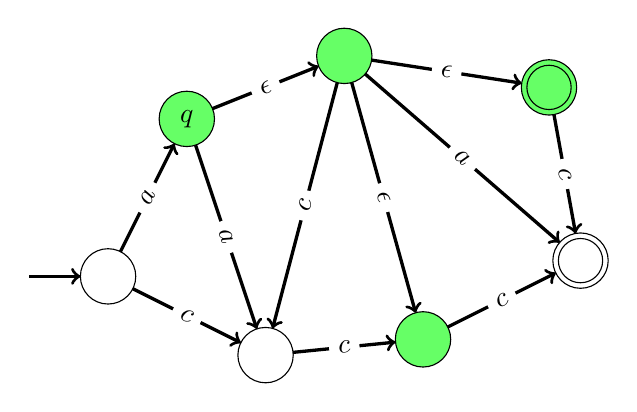
\begin{tikzpicture}[
  vertex/.style = {
    shape = circle,
    draw = black,
    minimum size = 20pt,
    inner sep = 0pt,
    outer sep = 0pt,
  }
]
  \node[vertex] (v1) at (1, 0) {};
  \node[vertex, fill = green!60] (v2) at (2, 2) {\(q\)};
  \node[vertex, fill = green!60] (v3) at (4, 2.8) {};
  \node[vertex, fill = green!60] (v4) at (6.6,  2.4) {};
  \node[vertex] (v5) at (7, 0.2) {};
  \node[vertex, fill = green!60] (v6) at (5, -0.8) {};
  \node[vertex] (v7) at (3, -1) {};

  \draw (6.6, 2.4) circle (8pt);
  \draw (7, 0.2) circle (8pt);

  \begin{scope}[
    every path/.style = {->, very thick },
    every node/.style = { midway, sloped, fill = white }
  ]
    \draw (0, 0) -- (v1);
    \draw (v1) -- (v2) node {\(a\)};
    \draw (v1) -- (v7) node {\(c\)};

    \draw (v2) -- (v3) node {\(\epsilon\)};
    \draw (v2) -- (v7) node {\(a\)};

    \draw (v3) -- (v4) node {\(\epsilon\)};
    \draw (v3) -- (v5) node {\(a\)};
    \draw (v3) -- (v6) node {\(\epsilon\)};
    \draw (v3) -- (v7) node {\(c\)};

    \draw (v4) -- (v5) node {\(c\)};

    \draw (v6) -- (v5) node {\(c\)};

    \draw (v7) -- (v6) node {\(c\)};
  \end{scope}
\end{tikzpicture}
